\section{Bakti Qilan Mufid | 1174083}
\subsection{Buatlah library fungsi (file terpisah/library dengan nama NPM\textunderscore bar.py) untuk plot dengan jumlah subplot adalah NPM mod 3 + 2}
\hfill \break
Pertama-tama kita harus mengetahui hasil dari NPM mod 3 + 2 terlebih dahulu, lalu sesudah itu kita membuat subplotnya, seperti pada kode berikut:
\lstinputlisting[firstline=9, lastline=79]{src/6/1174083/Praktek/1174083_bar.py}

\subsection{Buatlah library fungsi (file terpisah/library dengan nama NPM\textunderscore scatter.py) untuk plot dengan jumlah subplot adalah NPM mod 3 + 2}
\hfill \break
Pertama-tama kita harus mengetahui hasil dari NPM mod 3 + 2 terlebih dahulu, lalu sesudah itu kita membuat subplotnya, seperti pada kode berikut:
\lstinputlisting[firstline=9, lastline=79]{src/6/1174083/Praktek/1174083_scatter.py}

\subsection{Buatlah library fungsi (file terpisah/library dengan nama NPM\textunderscore pie.py) untuk plot dengan jumlah subplot adalah NPM mod 3 + 2}
\hfill \break
Pertama-tama kita harus mengetahui hasil dari NPM mod 3 + 2 terlebih dahulu, lalu sesudah itu kita membuat subplotnya, seperti pada kode berikut:
\lstinputlisting[firstline=9, lastline=54]{src/6/1174083/Praktek/1174083_pie.py}

\subsection{Buatlah library fungsi (file terpisah/library dengan nama NPM\textunderscore plot.py) untuk plot dengan jumlah subplot adalah NPM mod 3 + 2}
\hfill \break
Pertama-tama kita harus mengetahui hasil dari NPM mod 3 + 2 terlebih dahulu, lalu sesudah itu kita membuat subplotnya, seperti pada kode berikut:
\lstinputlisting[firstline=9, lastline=79]{src/6/1174083/Praktek/1174083_plot.py}

\subsection{Keterampilan Penanganan Error}
Fungsi Penanganan error sebagai berikut:
\lstinputlisting[firstline=9, lastline=26]{src/6/1174083/Praktek/error.py}

%%%%%%%%%%%%%%%%%%%%%%%%%%%%%%%%%%%%%%%%%%%%%%%%%%%%%%%%%%%%%%%%%%%%%%%%%%%%%%%%%%%%%%%%%%%%%%%%%%%%%%%%%%%%%%%%
\section{Mochamad Arifqi Ramadhan | 1174074}
\subsection{Keterampilan Pemograman }
\subsubsection{Buatlah library fungsi (file terpisah/library dengan nama NPM/textunderscore bar.py) untuk plot dengan jumlah subplot adalah NPM mod 3 + 2}

Ini adalah fungsi untuk membuat plot bar sesuai dengan hasil modulus:
\lstinputlisting[firstline=7, lastline=44]{src/6/1174074/Praktek/a1174074_bar.py}

Berikut ini cara pemanggilannya:
\lstinputlisting[firstline=7, lastline=21]{src/6/1174074/Praktek/main.py}

\subsubsection{Buatlah library fungsi (file terpisah/library dengan nama NPM/textunderscore scatter.py) untuk plot dengan jumlah subplot adalah NPM mod 3 + 2}

Ini adalah fungsi untuk membuat plot scatter sesuai dengan hasil modulus:
\lstinputlisting[firstline=7, lastline=44]{src/6/1174074/Praktek/a1174074_scatter.py}

Berikut ini cara pemanggilannya:
\lstinputlisting[firstline=23, lastline=37]{src/6/1174074/Praktek/main.py}

\subsubsection{Buatlah library fungsi (file terpisah/library dengan nama NPM/textunderscore pie.py) untuk plot dengan jumlah subplot adalah NPM mod 3 + 2}

Ini adalah fungsi untuk membuat plot pie sesuai dengan hasil modulus:
\lstinputlisting[firstline=8, lastline=52]{src/6/1174074/Praktek/a1174074_pie.py}

Berikut ini cara pemanggilannya:
\lstinputlisting[firstline=39, lastline=53]{src/6/1174074/Praktek/main.py}

\subsubsection{Buatlah library fungsi (file terpisah/library dengan nama NPM/textunderscore pie.py) untuk plot dengan jumlah subplot adalah NPM mod 3 + 2}

Ini adalah fungsi untuk membuat subplot sesuai dengan hasil modulus:
\lstinputlisting[firstline=7, lastline=44]{src/6/1174074/Praktek/a1174074_plot.py}

Berikut ini cara pemanggilannya:
\lstinputlisting[firstline=55, lastline=69]{src/6/1174074/Praktek/main.py}


\subsubsection{Keterampilan Penanganan Error}
\lstinputlisting[firstline=7, lastline=19]{src/6/1174074/Praktek/1174074_error.py}
%%%%%%%%%%%%%%%%%%%%%%%%%%%%%%%%%%%%%%%%%%%%%%%%%%%%%%%%%%%%%%%%%%%%%%%%%%%%%%%%%%%%%%%%%%%%%%%%%%%%%%%%%%%%%%%%%%%%%%%%%%%%%%%%%%
\section{Advent Nopele Olansi Damiahan Sihite / 1174089)}
\subsection{Teori}
\subsubsection{Soal No. 1}
\hfill \break
Apa itu fungsi library matplotlib?

\hfill \break
Matplotlib merupakan salah satu library Python 2D yang dapat menghasilkan plot dengan kualitas yang tinggi dalam berbagai format dan dapat digunakan di berbagai platform. Matplotlib berfungsi sebagai pembuat grafik di berbagai platform, seperti Python dan Jupyter. Grafik yang dibuat menggunakan Matplotlib bisa dibuat dalam berbagai bentuk, seperti grafik garis, batang, lingkaran, histogram, dan sebagainya.

\subsubsection{Soal No. 2}
\hfill \break
Jelaskan langkah-langkah membuat sumbu X dan Y di matplotlib!

\begin{enumerate}
	\item Pertama import library Matplotlib.	
	\lstinputlisting[firstline=2, lastline=2]{src/6/1174089/Praktek/1174089.py}
	
	\item Buat variabel x yang menampung list untuk sumbu x dan variabel y yang menampung list untuk sumbu y.	
	\lstinputlisting[firstline=4, lastline=5]{src/6/1174089/Praktek/1174089.py}
	
	\item Panggil fungsi plot dan isi parameter pertama dengan variabel x dan parameter kedua dengan variabel y.
	\lstinputlisting[firstline=7, lastline=7]{src/6/1174089/Praktek/1174089.py}	

	\item Lalu panggil plot tadi dengan memanggil fungsi show.
	\lstinputlisting[firstline=9, lastline=9]{src/6/1174089/Praktek/1174089.py}
	
\end{enumerate}
\hfill \break
\textbf{Kode Program}

\lstinputlisting[caption = Kode program membuat diagram menggunakan Matplotlib., firstline=2, lastline=9]{src/6/1174089/Praktek/1174089.py}

\hfill \break
\textbf{Hasil Compile}

\begin{figure}[H]
	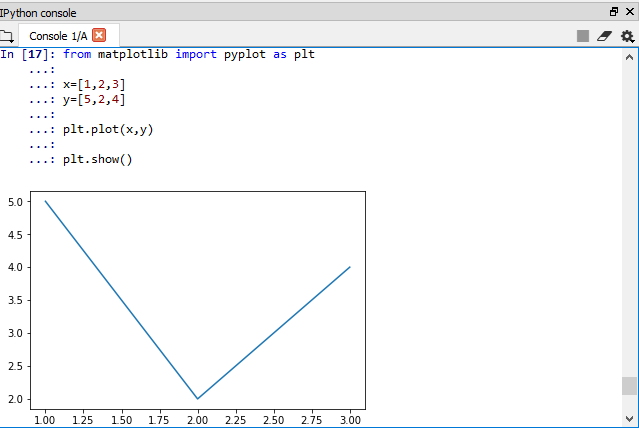
\includegraphics[width=12cm]{figures/6/1174089/Praktek/2.png}
	\centering
	\caption{Hasil compile membuat diagram menggunakan Matplotlib.}
\end{figure}
 
\subsubsection{Soal No. 3}
\hfill \break
Jelaskan bagaimana perbedaan fungsi dan cara pakai untuk berbagai jenis(bar, histogram ,scatter ,line, dll) jenis plot di matplotlib!

\begin{enumerate}
	\item \textbf{Bar Graph}
	
	Perbedaan bar graph dengan jenis plot yang lain adalah bar graph menggunakan bar atau batang-batang untuk membandingkan data di antara berbagai kategori.
	
	\textbf{Kode Program}
	
	\lstinputlisting[caption = Kode program membuat bar graph menggunakan Matplotlib., firstline=13, lastline=25]{src/6/1174089/Praktek/1174089.py}
	
	\textbf{Hasil Compile}
	
	\begin{figure}[H]
		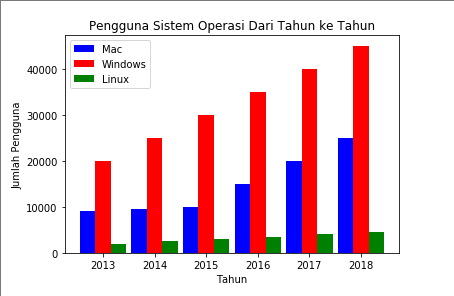
\includegraphics[width=12cm]{figures/6/1174089/Praktek/bar.png}
		\centering
		\caption{Hasil compile membuat bar graph menggunakan Matplotlib.}
	\end{figure}
	
	\item \textbf{Histogram}
	
	Perbedaan histogram dengan jenis plot yang lain adalah histogram akan membuat plot dimana plot yang dimunculkan merupakan gabungan dari beberapa data yang telah dikelompokkan.
	
	\textbf{Kode Program}
	
	\lstinputlisting[caption = Kode program membuat histogram menggunakan Matplotlib., firstline=29, lastline=36]{src/6/1174089/Praktek/1174089.py}
	
	\textbf{Hasil Compile}
	
	\begin{figure}[H]
		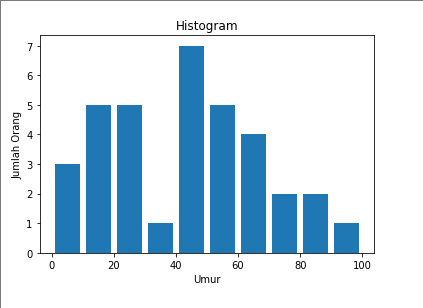
\includegraphics[width=12cm]{figures/6/1174089/Praktek/histogram.png}
		\centering
		\caption{Hasil compile membuat histogram menggunakan Matplotlib.}
	\end{figure}
	
	\item \textbf{Scatter Plot}
	
	Perbedaan scatter plot dengan jenis plot lain adalah scatter plot menampilkan data sebagai kumpulan titik, masing-masing memiliki nilai satu variabel yang menentukan posisi pada sumbu horizontal dan nilai variabel lain menentukan posisi pada sumbu vertikal.
	
	\textbf{Kode Program}
	
	\lstinputlisting[caption = Kode program membuat scatter plot menggunakan Matplotlib., firstline=40, lastline=53]{src/6/1174089/Praktek/1174089.py}
	
	\textbf{Hasil Compile}
	
	\begin{figure}[H]
		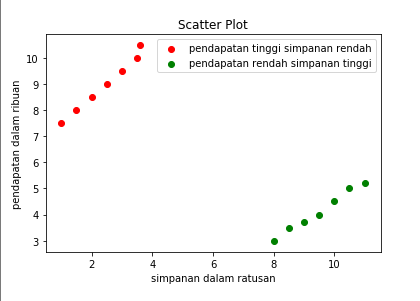
\includegraphics[width=12cm]{figures/6/1174089//Praktek/scatter.png}
		\centering
		\caption{Hasil compile membuat scatter plot menggunakan Matplotlib.}
	\end{figure}
	
	\item \textbf{Area Plot}
	
	Perbedaan area plot dengan jenis plot lain adalah area plot digunakan untuk melacak perubahan dari waktu ke waktu untuk dua atau lebih kelompok terkait yang membentuk satu kategori secara keseluruhan.
	
	\textbf{Kode Program}
	
	\lstinputlisting[caption = Kode program membuat diagram menggunakan Matplotlib., firstline=57, lastline=76]{src/6/1174089/Praktek/1174089.py}
	
	\textbf{Hasil Compile}
	
	\begin{figure}[H]
		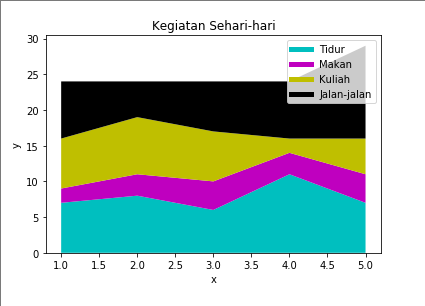
\includegraphics[width=12cm]{figures/6/1174089/Praktek/area.png}
		\centering
		\caption{Hasil compile membuat diagram menggunakan Matplotlib.}
	\end{figure}
	
	\item \textbf{Pie Plot}
	
	Perbedaan pie plot dengan jenis plot lain adalah pie plot digunakan untuk menunjukkan persentase atau data proporsional di mana setiap potongan pie mewakili kategori.
	
	\textbf{Kode Program}
	
	\lstinputlisting[caption = Kode program membuat Pie Plot menggunakan Matplotlib., firstline=86, lastline=101]{src/6/1174089/Praktek/1174089.py}
	
	\textbf{Hasil Compile}
	
	\begin{figure}[H]
		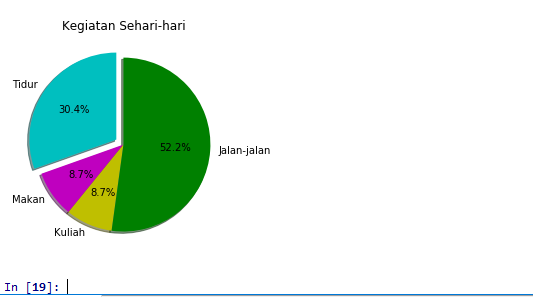
\includegraphics[width=9cm]{figures/6/1174089/Praktek/pie.png}
		\centering
		\caption{Hasil compile membuat Pie Plot menggunakan Matplotlib.}
	\end{figure}
	
	\item \textbf{Line Graph}
	
	Perbedaan line graph dengan jenis plot lain adalah line graph menampilkan diagram dalam bentuk garis.
	
	\textbf{Kode Program}
	
	\lstinputlisting[caption = Kode program membuat diagram menggunakan Matplotlib., firstline=105, lastline=113]{src/6/1174089/Praktek/1174089.py}
	
	\textbf{Hasil Compile}
	
	\begin{figure}[H]
		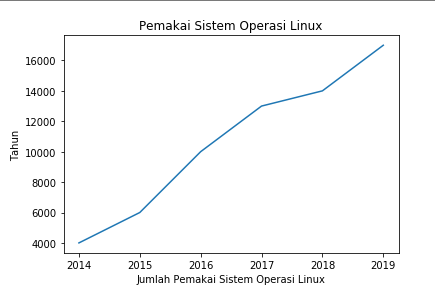
\includegraphics[width=12cm]{figures/6/1174089/Praktek/line.png}
		\centering
		\caption{Hasil compile membuat diagram menggunakan Matplotlib.}
	\end{figure}
	
\end{enumerate}

\subsubsection{Soal No. 4}
\hfill \break
Jelaskan bagaimana cara menggunakan legend dan label serta kaitannya dengan fungsi tersebut!

\begin{enumerate}
	\item Untuk menggunakan legend definisikan parameter label di tiap fungsi plot. Parameter label digunakan untuk memberikan label pada line sebagai pembeda antar line.
	
	\lstinputlisting[caption = Kode program menggunakan parameter label dengan Matplotlib., firstline=123, lastline=124]{src/6/1174089/Praktek/1174089.py}
	
	\item Kemudian panggil fungsi legend.
	
	\lstinputlisting[caption = Kode program memanggil fungsi legend dengan Matplotlib., firstline=128, lastline=128]{src/6/1174089/Praktek/1174089.py}
\end{enumerate}

\hfill \break
\textbf{Kode Program}

\lstinputlisting[caption = Kode program membuat diagram menggunakan Matplotlib., firstline=117, lastline=130]{src/6/1174089/Praktek/1174089.py}

\hfill \break
\textbf{Hasil Compile}

\begin{figure}[H]
	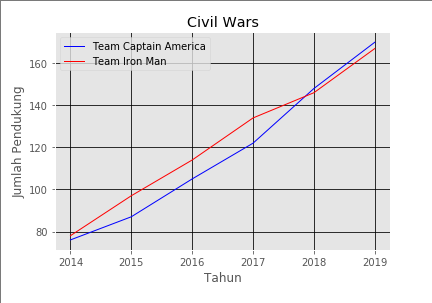
\includegraphics[width=12cm]{figures/6/1174089/Praktek/4.png}
	\centering
	\caption{Hasil compile membuat diagram menggunakan Matplotlib.}
\end{figure}

\subsubsection{Soal No. 5}
\hfill \break
Jelaskan apa fungsi dari subplot di matplotlib, dan bagaimana cara kerja dari fungsi subplot, sertakan ilustrasi dan gambar sendiri dan apa parameternya jika ingin menggambar plot dengan 9 subplot di dalamnya!

\hfill \break
Fungsi subplot adalah untuk membuat beberapa plot di dalam satu gambar.
\hfill \break
Cara kerja subplot, yaitu fungsi subplot memiliki parameter pertama adalah jumlah kolom, parameter kedua adalah jumlah baris, dan parameter ketiga adalah index plot keberapanya.

\hfill \break
\textbf{Kode Program}

\lstinputlisting[caption = Kode program membuat subplot menggunakan Matplotlib., firstline=134, lastline=146]{src/6/1174089/Praktek/1174089.py}

\hfill \break
\textbf{Hasil Compile}

\begin{figure}[H]
	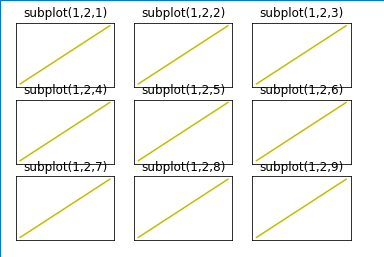
\includegraphics[width=12cm]{figures/6/1174089/Praktek/subplot.png}
	\centering
	\caption{Hasil compile membuat subplot menggunakan Matplotlib.}
\end{figure}

\subsubsection{Soal No. 6}
\hfill \break
Sebutkan semua parameter color yang bisa digunakan (contoh:  m,c,r,k,...  dkk)!

\begin{itemize}
	\item 'b' (blue)
	\item 'g' (green)
	\item 'r' (red)
	\item 'c' (cyan)
	\item 'm' (magenta)
	\item 'y' (yellow)
	\item 'k' (black)
	\item 'w' (white)
\end{itemize}

\subsubsection{Soal No. 7}
\hfill \break
Jelaskan bagaimana cara kerja dari fungsi hist, sertakan ilustrasi dan gambar sendiri!

\hfill \break
Cara kerja dari fungsi hist yaitu fungsi hist akan menerima parameter yang diberikan, kemudian fungsi hist akan dieksekusi sesuai dengan parameter yang diberikan.

\hfill \break
\textbf{Kode Program}

\lstinputlisting[caption = Kode program membuat diagram menggunakan Matplotlib., firstline=150, lastline=157]{src/6/1174089/Praktek/1174089.py}

\hfill \break
\textbf{Hasil Compile}

\begin{figure}[H]
	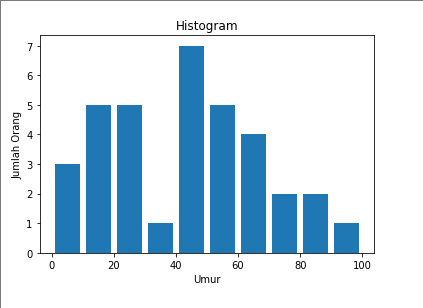
\includegraphics[width=12cm]{figures/6/1174089/Praktek/histogram.png}
	\centering
	\caption{Hasil compile membuat diagram menggunakan Matplotlib.}
\end{figure}

\subsubsection{Soal No. 8}
\hfill \break
 Jelaskan lebih mendalam tentang parameter dari fungsi pie diantaranya labels, colors, startangle, shadow, explode, autopct!
 
 \begin{itemize}
 	\item labels : untuk memberikan label di tiap persentase.
 	\item colors : untuk memberikan warna di tiap persentase.
 	\item startangle : untuk memutar plot sesuai dengan derajat yang ditentukan.
 	\item shadow : untuk memberikan bayangan pada plot.
 	\item explode : untuk memisahkan antar tiap potongan pie pada plot.
 	\item autopct : untuk menentukan jumlah angka dibelakang koma.
 \end{itemize}

\subsection{Praktek}
\subsubsection{Soal No. 1}
\hfill \break
Buatlah librari fungsi (file terpisah/library dengan nama NPMbar.py) untuk plot dengan jumlah subplot adalah NPM mod 3 + 2!

\hfill \break
\textbf{Kode Program}

\lstinputlisting[caption = Kode program membuat fungsi Bar Plot menggunakan Matplotlib., firstline=1, lastline=21]{src/6/1174089/Praktek/1174089_bar.py}

\hfill \break
\textbf{Hasil Compile}

\begin{figure}[H]
	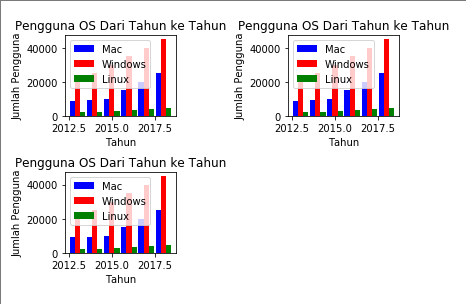
\includegraphics[width=12cm]{figures/6/1174089/Praktek/p1.png}
	\centering
	\caption{Hasil compile membuat fungsi Bar Plot menggunakan Matplotlib.}
\end{figure}

\subsubsection{Soal No. 2}
\hfill \break
Buatlah librari fungsi (file terpisah/library dengan nama NPMscatter.py) untuk plot dengan jumlah subplot NPM mod 3 + 2!

\hfill \break
\textbf{Kode Program}

\lstinputlisting[caption = Kode program membuat fungsi Scatter Plot menggunakan Matplotlib., firstline=1, lastline=23]{src/6/1174089/Praktek/1174089_scatter.py}

\hfill \break
\textbf{Hasil Compile}

\begin{figure}[H]
	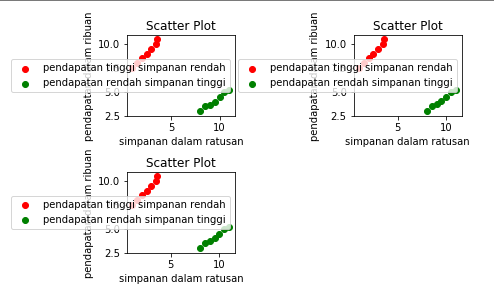
\includegraphics[width=12cm]{figures/6/1174089/Praktek/p2.png}
	\centering
	\caption{Hasil compile membuat fungsi Scatter Plot menggunakan Matplotlib.}
\end{figure}

\subsubsection{Soal No. 3}
\hfill \break
Buatlah librari fungsi (file terpisah/library dengan nama NPMpie.py) untuk plot dengan jumlah subplot NPM mod 3 + 2!

\hfill \break
\textbf{Kode Program}

\lstinputlisting[caption = Kode program membuat fungsi Pie Plot menggunakan Matplotlib., firstline=1, lastline=23]{src/6/1174089/Praktek/1174089_pie.py}

\hfill \break
\textbf{Hasil Compile}

\begin{figure}[H]
	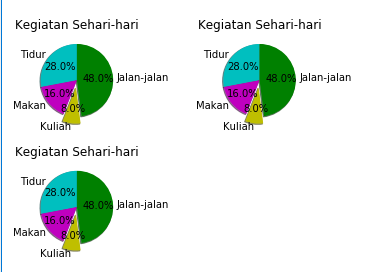
\includegraphics[width=12cm]{figures/6/1174089/Praktek/p3.png}
	\centering
	\caption{Hasil compile membuat fungsi Pie Plot menggunakan Matplotlib.}
\end{figure}

\subsubsection{Soal No. 4}
\hfill \break
Buatlah librari fungsi (file terpisah/library dengan nama NPMplot.py) untuk plot dengan jumlah subplot NPM mod 3 + 2

\hfill \break
\textbf{Kode Program}

\lstinputlisting[caption = Kode program membuat fungsi Plot menggunakan Matplotlib., firstline=1, lastline=23]{src/6/1174089/Praktek/1174089_plot.py}

\hfill \break
\textbf{Hasil Compile}

\begin{figure}[H]
	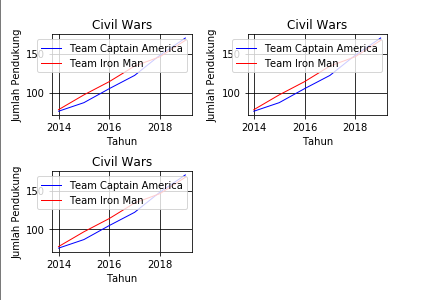
\includegraphics[width=12cm]{figures/6/1174089/Praktek/p4.png}
	\centering
	\caption{Hasil compile membuat fungsi Plot menggunakan Matplotlib.}
\end{figure}


\subsection{Penanganan Error}
Tuliskan  peringatan  error  yang  didapat  dari  mengerjakan  praktek  keenam  ini, dan  jelaskan  cara  penanganan  error  tersebut. dan  Buatlah  satu  fungsi  yang menggunakan try except untuk menanggulangi error tersebut.

\hfill \break
Peringatan error di praktek kelima ini, yaitu:
\begin{itemize}
	\item Syntax Errors
	Syntax Errors adalah suatu keadaan saat kode python mengalami kesalahan penulisan. Solusinya adalah memperbaiki penulisan kode yang salah.
	
	\item Name Error
	NameError adalah exception yang terjadi saat kode melakukan eksekusi terhadap local name atau global name yang tidak terdefinisi. Solusinya adalah memastikan variabel atau function yang dipanggil ada atau tidak salah ketik.
	
	\item Type Error
	TypeError adalah exception yang akan terjadi apabila pada saat dilakukannya eksekusi terhadap suatu operasi atau fungsi dengan type object yang tidak sesuai. Solusi dari error ini adalah mengkoversi varibelnya sesuai dengan tipe data yang akan digunakan.
\end{itemize}
\hfill \break
Fungsi yang menggunakan try except untuk menanggulangi error.

\hfill \break
\textbf{Kode Program}

\lstinputlisting[caption = Kode program membuat fungsi penanganan error., firstline=161, lastline=178]{src/6/1174089/Praktek/1174089.py}

\hfill \break
\textbf{Hasil Compile}

\begin{figure}[H]
	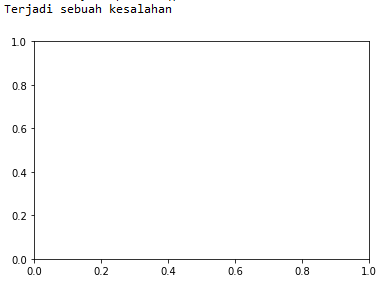
\includegraphics[width=12cm]{figures/6/1174089/Praktek/error.png}
	\centering
	\caption{Hasil compile membuat fungsi penanganan error.}
\end{figure}

\subsection{Screenshoot Plagiat}
\begin{figure}[H]
	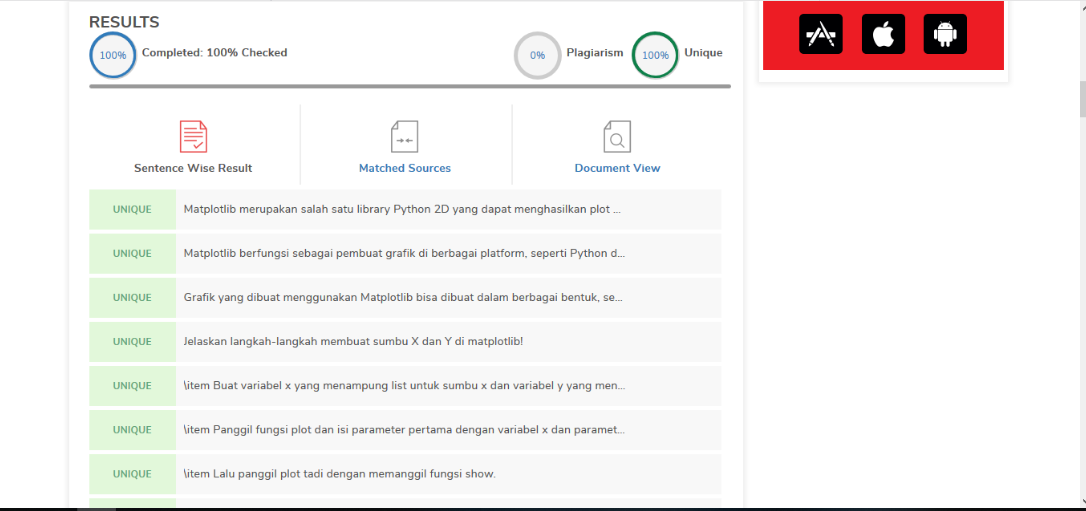
\includegraphics[width=12cm]{figures/6/1174089/Praktek/plagiat.png}
	\centering
\end{figure}
\subsection{Screenshoot Kode Program}
\begin{figure}[H]
	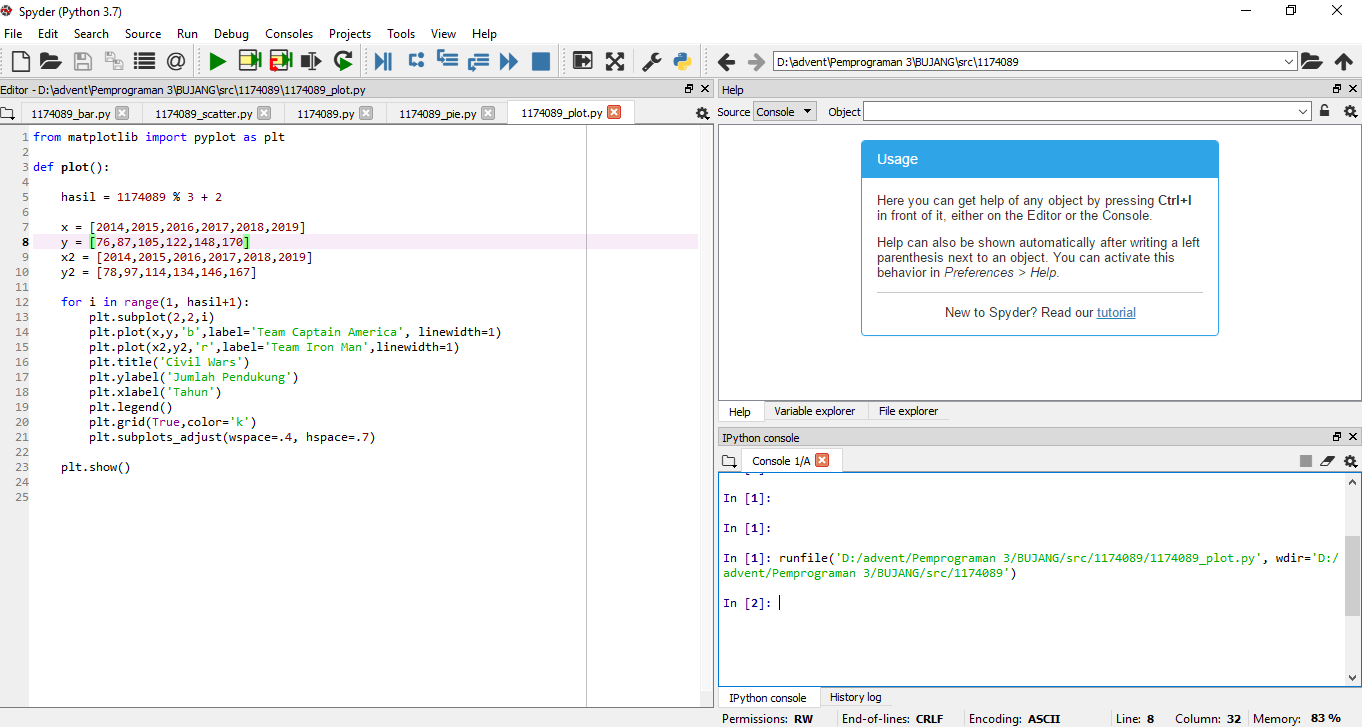
\includegraphics[width=9cm]{figures/6/1174089/Praktek/c1.png}
	\centering
\end{figure}
\begin{figure}[H]
	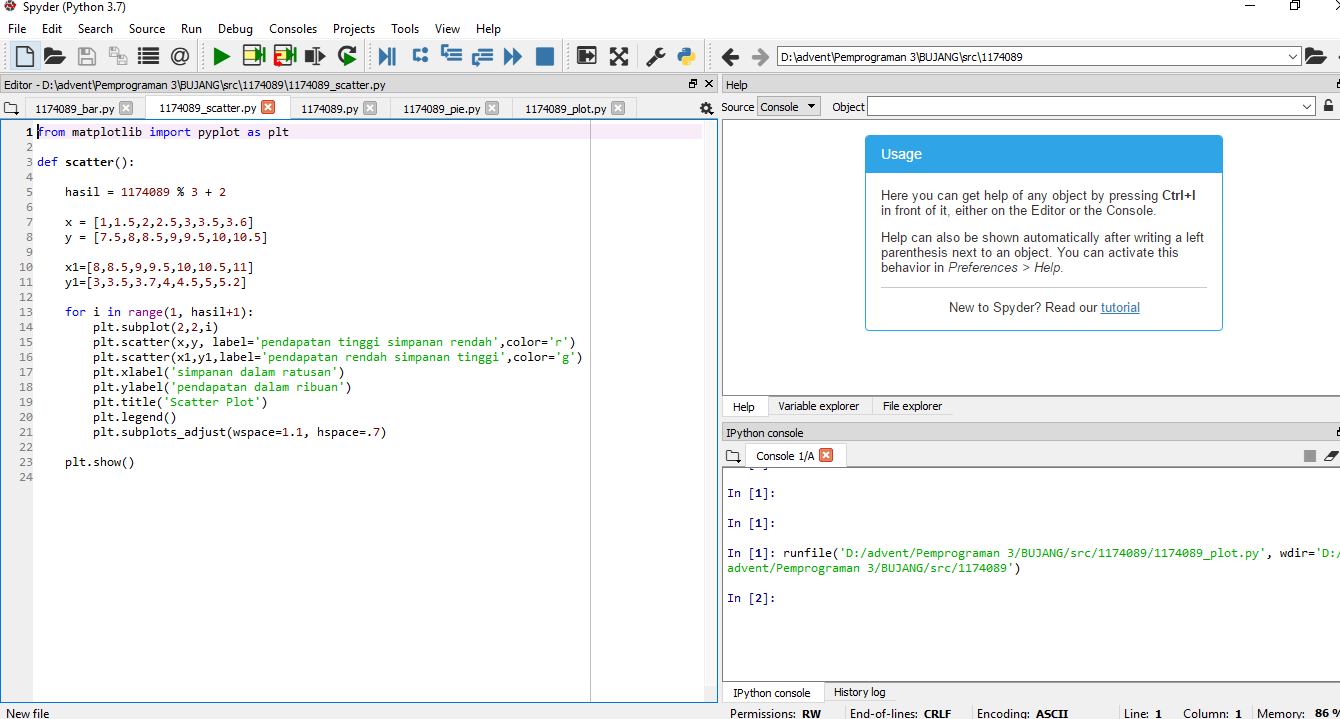
\includegraphics[width=9cm]{figures/6/1174089/Praktek/c2.png}
	\centering
\end{figure}
\begin{figure}[H]
	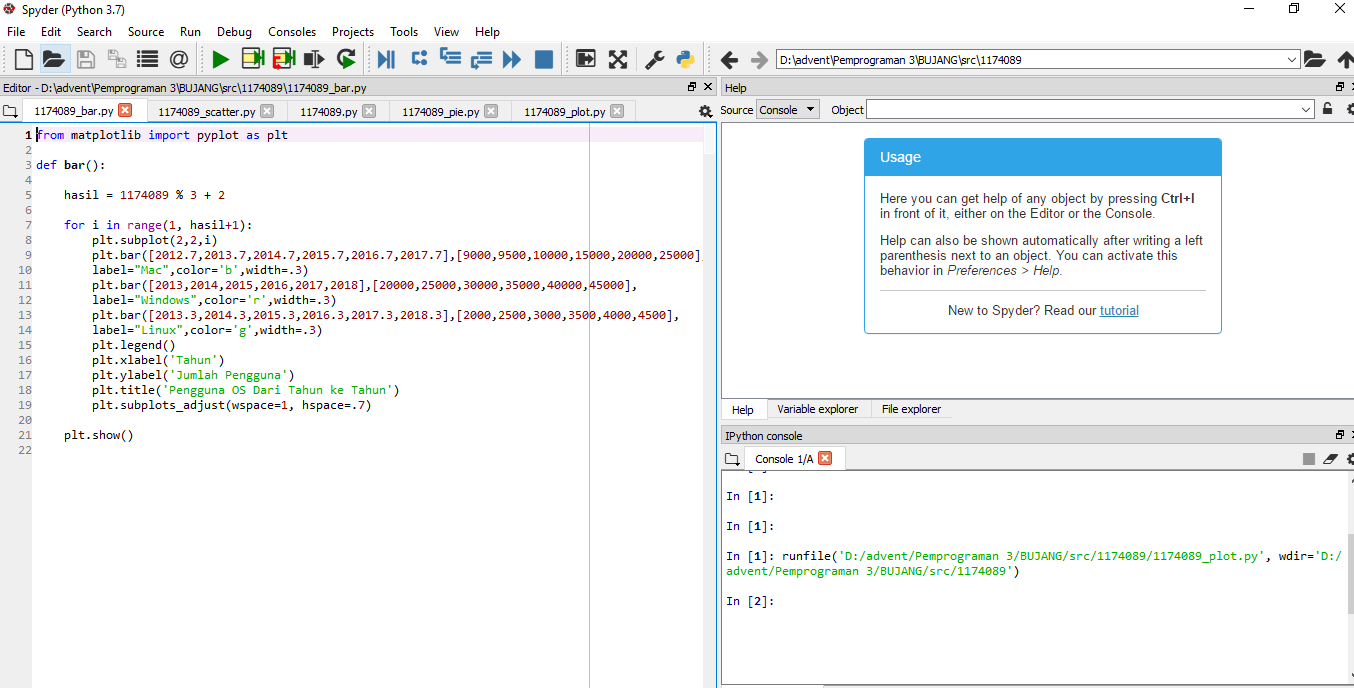
\includegraphics[width=9cm]{figures/6/1174089/Praktek/c3.png}
	\centering
\end{figure}
\begin{figure}[H]
	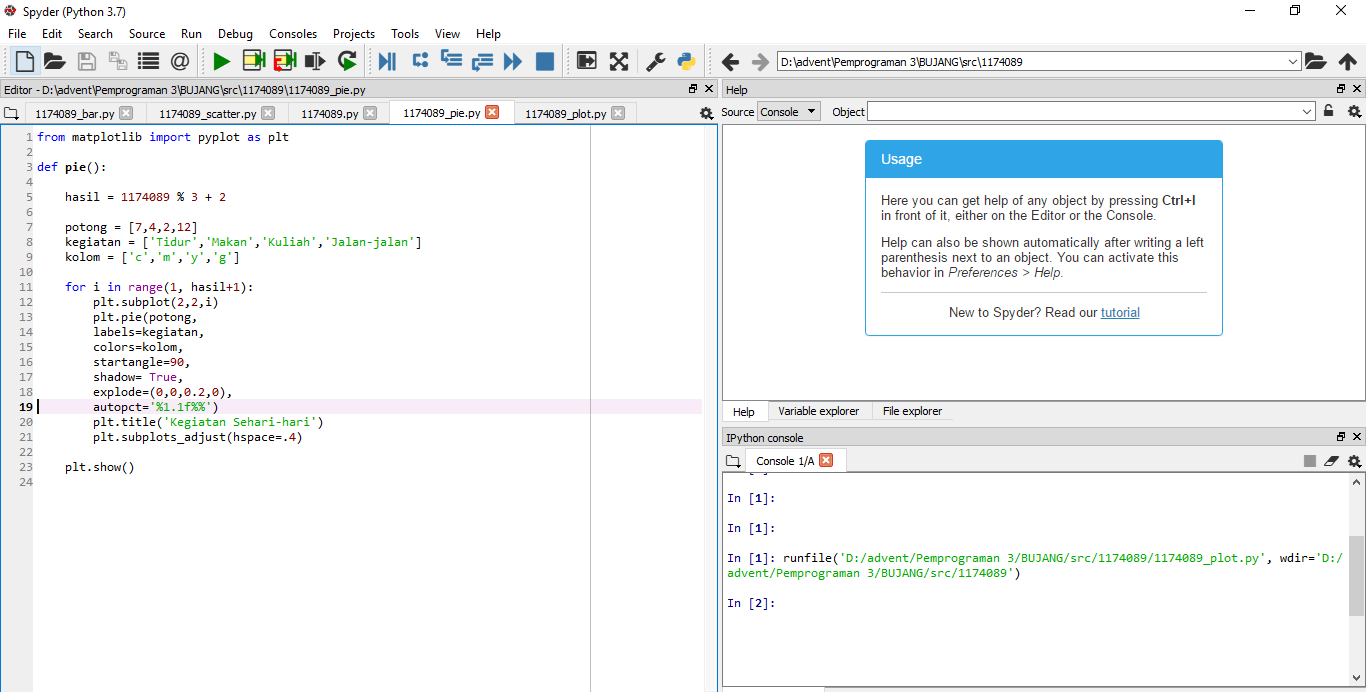
\includegraphics[width=9cm]{figures/6/1174089/Praktek/c4.png}
	\centering
\end{figure}
\begin{figure}[H]
	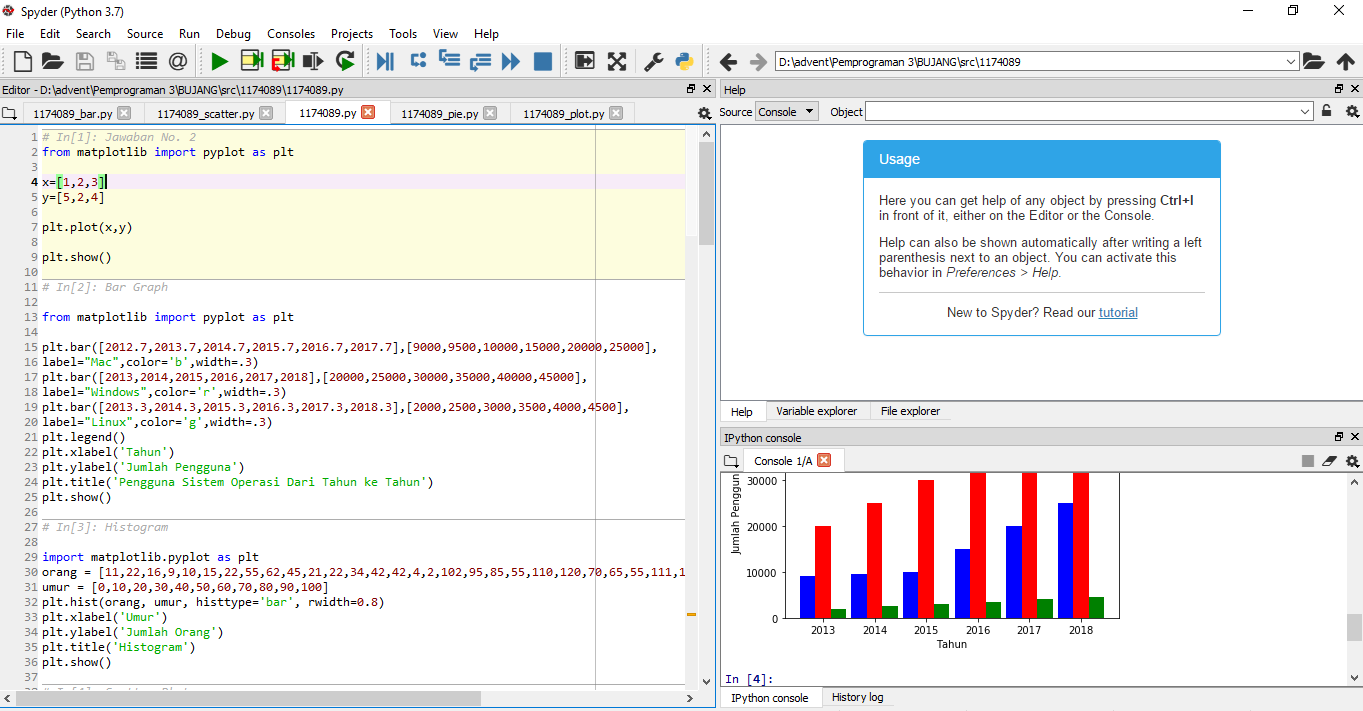
\includegraphics[width=9cm]{figures/6/1174089/Praktek/c5.png}
	\centering
\end{figure}
\begin{figure}[H]
	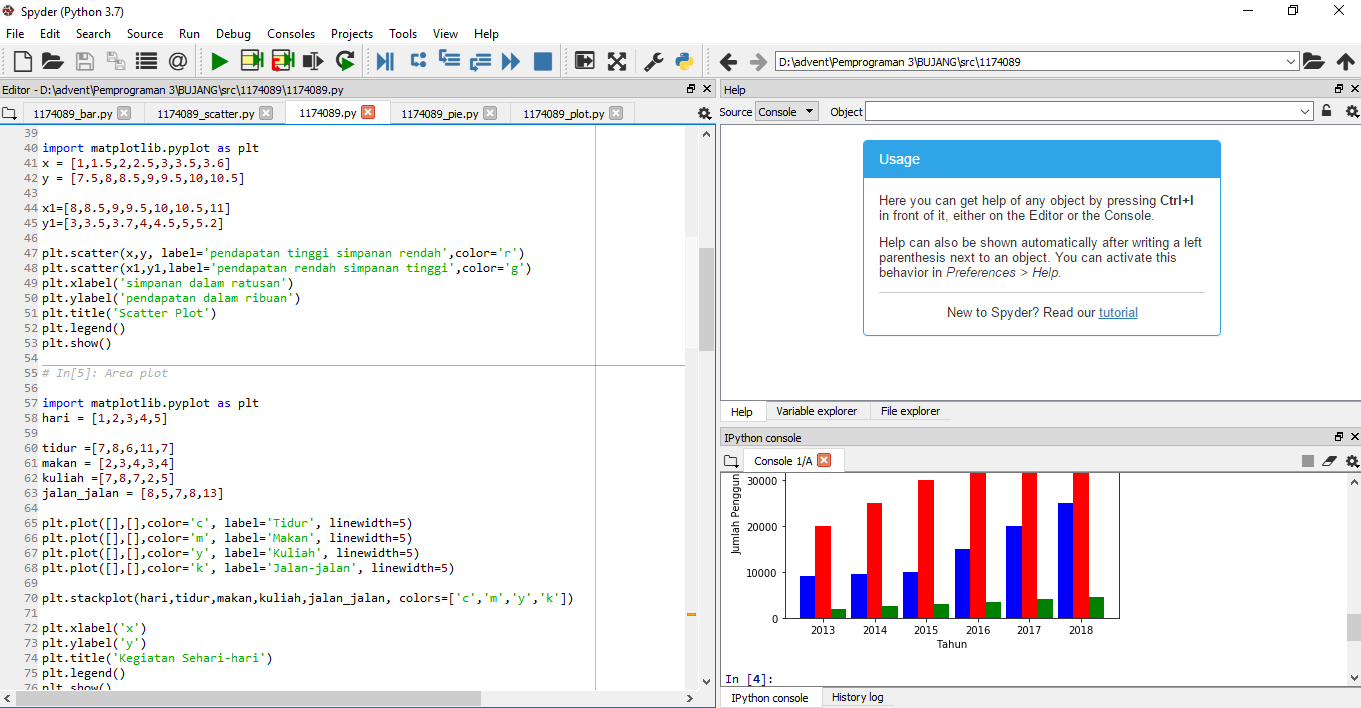
\includegraphics[width=9cm]{figures/6/1174089/Praktek/c6.png}
	\centering
\end{figure}
\begin{figure}[H]
	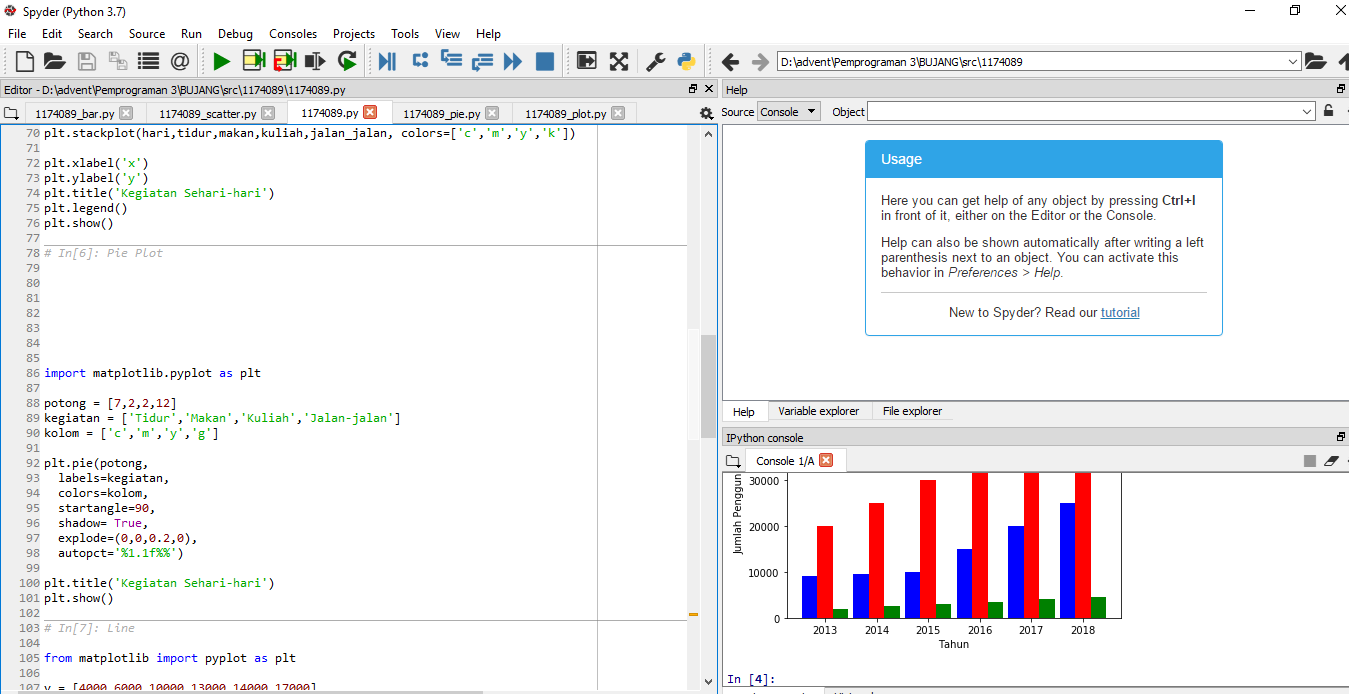
\includegraphics[width=9cm]{figures/6/1174089/Praktek/c7.png}
	\centering
\end{figure}
\begin{figure}[H]
	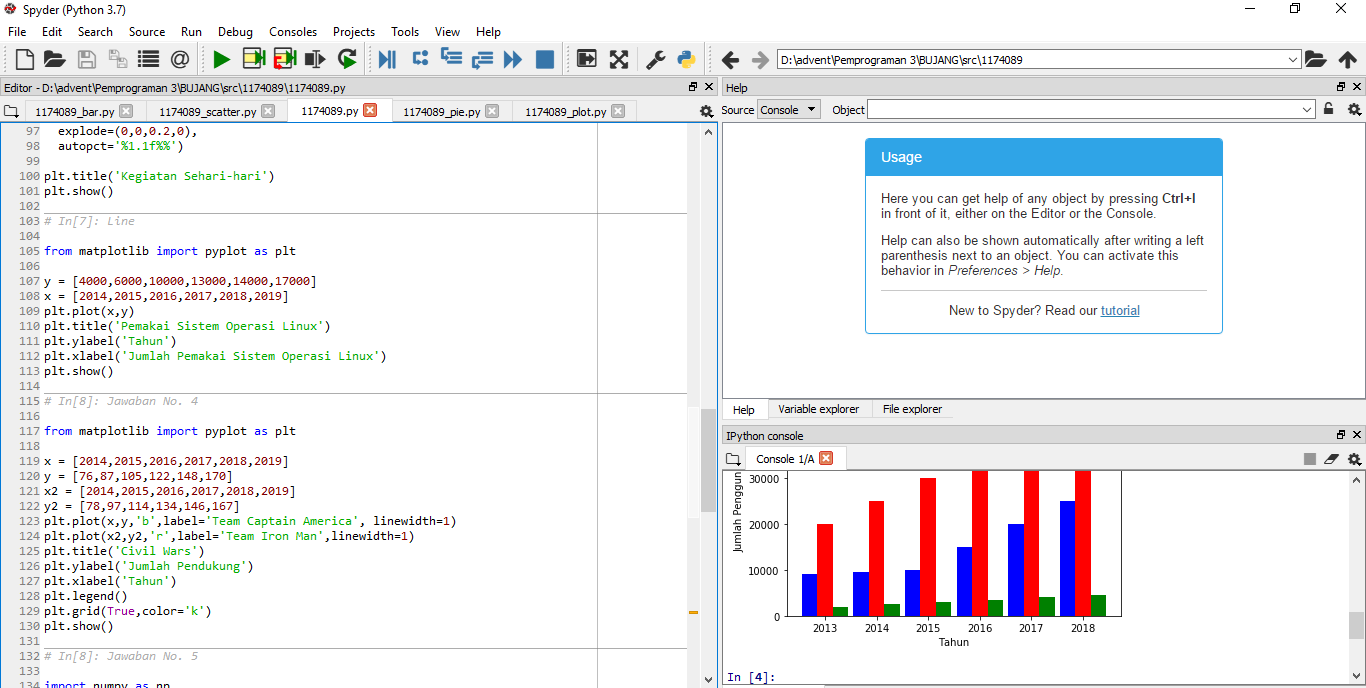
\includegraphics[width=9cm]{figures/6/1174089/Praktek/c8.png}
	\centering
\end{figure}
\begin{figure}[H]
	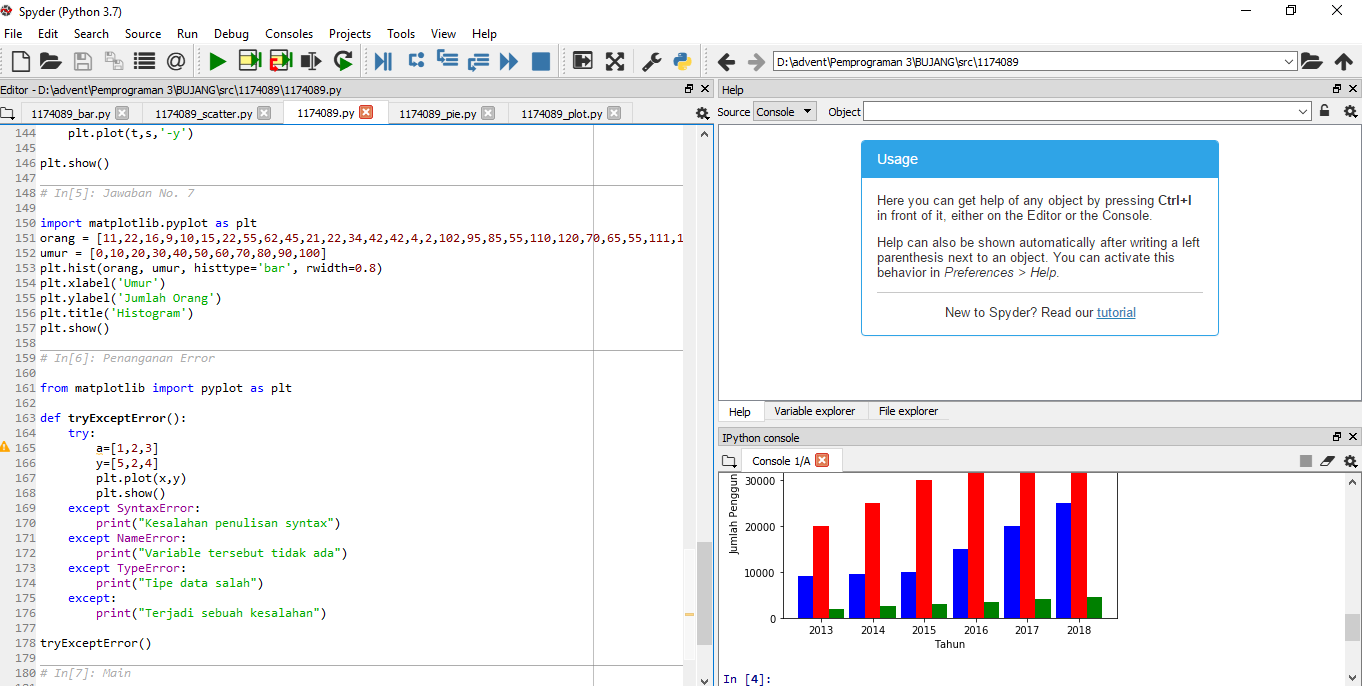
\includegraphics[width=9cm]{figures/6/1174089/Praktek/c9.png}
	\centering
\end{figure}
\begin{figure}[H]
	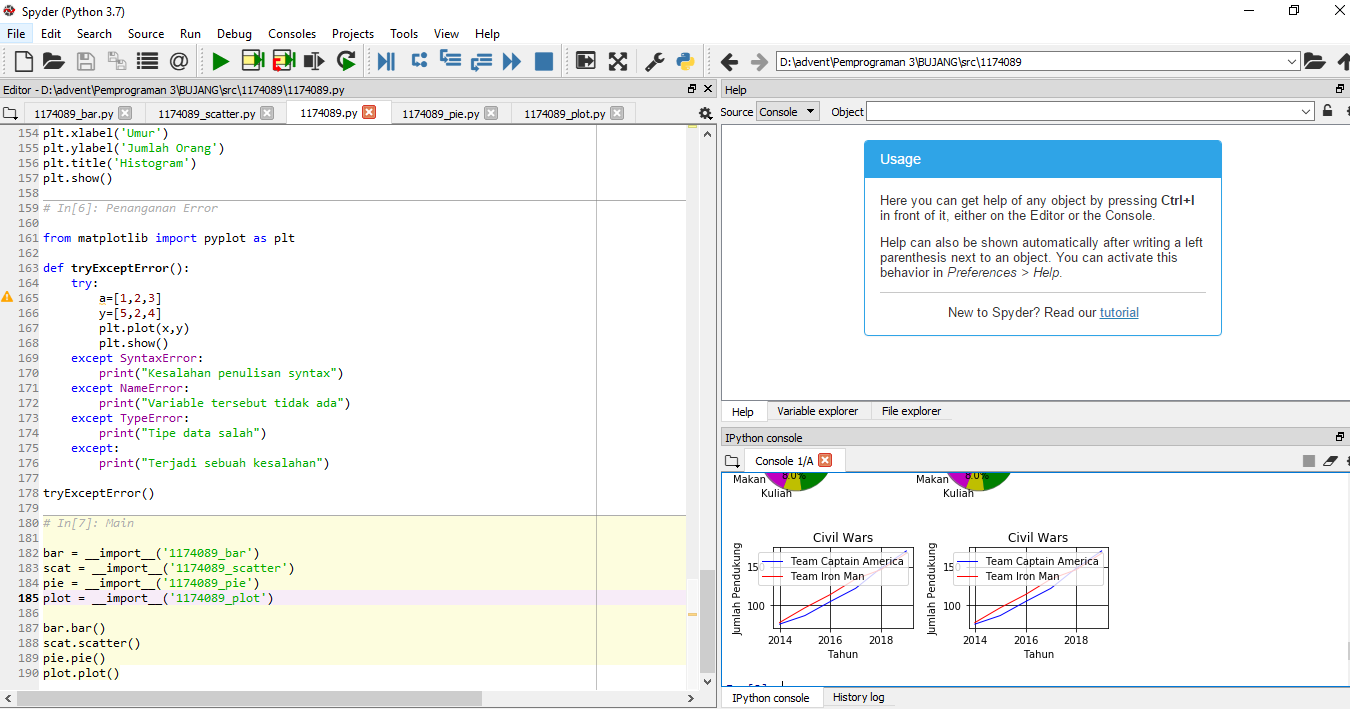
\includegraphics[width=9cm]{figures/6/1174089/Praktek/c10.png}
	\centering
\end{figure}
%%%%%%%%%%%%%%%%%%%%%%%%%%%%%%%%%%%%%%%%%%%%%%%%%%%%%%%%%%%%%%%%%

\section{Ilham Muhammad Ariq}
\subsection{Keterampilan Pemrograman}
\begin{enumerate}
\item Buatlah librari fungsi (file terpisah/library dengan nama \verb|NPM_bar.py|) untuk plot dengan jumlah subplot adalah NPM mod 3 + 2

	\lstinputlisting[firstline=8, lastline=30]{src/6/1174087/Praktek/1174087_bar.py}
	
\item Buatlah librari fungsi (file terpisah/library dengan nama \verb|NPM_scatter.py|) untuk plot dengan jumlah subplot NPM mod 3 + 2

	\lstinputlisting[firstline=8, lastline=30]{src/6/1174087/Praktek/1174087_scatter.py}

\item Buatlah librari fungsi (file terpisah/library dengan nama \verb|NPM_pie.py|) untuk plot dengan jumlah subplot NPM mod 3 + 2

	\lstinputlisting[firstline=8, lastline=52]{src/6/1174087/Praktek/1174087_pie.py}
	
\item  Buatlah librari fungsi (file terpisah/library dengan nama \verb|NPM_plot.py|) untuk plot dengan jumlah subplot NPM mod 3 + 2

	\lstinputlisting[firstline=8, lastline=30]{src/6/1174087/Praktek/1174087_plot.py}
	 
\end{enumerate}

\subsection{Keterampilan Penanganan Error}
\begin{enumerate}
\item Tuliskan peringatan error yang didapat dari mengerjakan praktek ketiga ini, dan jelaskan cara penanganan error tersebut. dan Buatlah satu fungsi yang menggunakan gunakan try except untuk menanggulangi error tersebut.

	\lstinputlisting[firstline=8, lastline=20]{src/6/1174087/Praktek/1174087_error.py}

\end{enumerate}

\textbf{Screenshoot Kode Program}
\begin{figure}[ht]	
    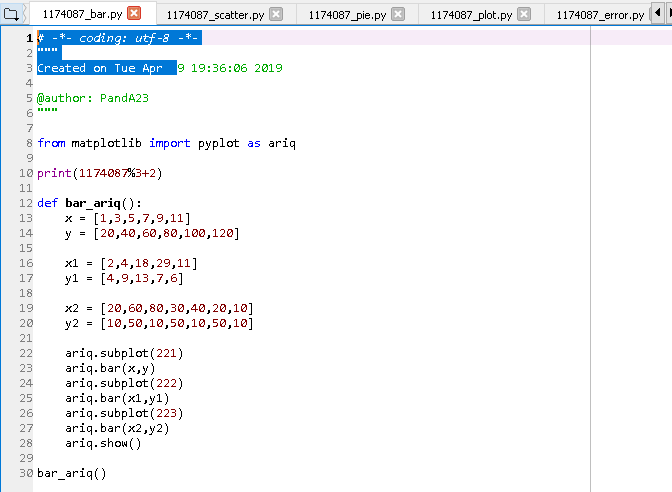
\includegraphics[width=7cm]{figures/6/1174087/Praktek/1174087_bar.png}
    \centering
    \caption{Bar}
\end{figure}

\begin{figure}[ht]	
    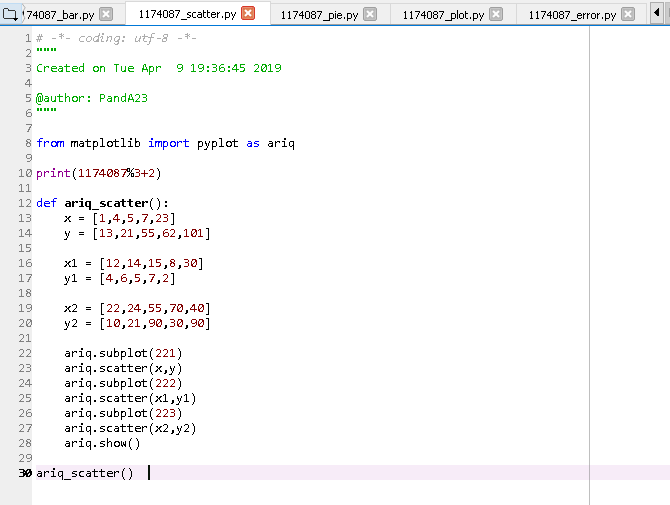
\includegraphics[width=7cm]{figures/6/1174087/Praktek/1174087_scatter.png}
    \centering
    \caption{Scatter}
\end{figure}

\begin{figure}[ht]	
    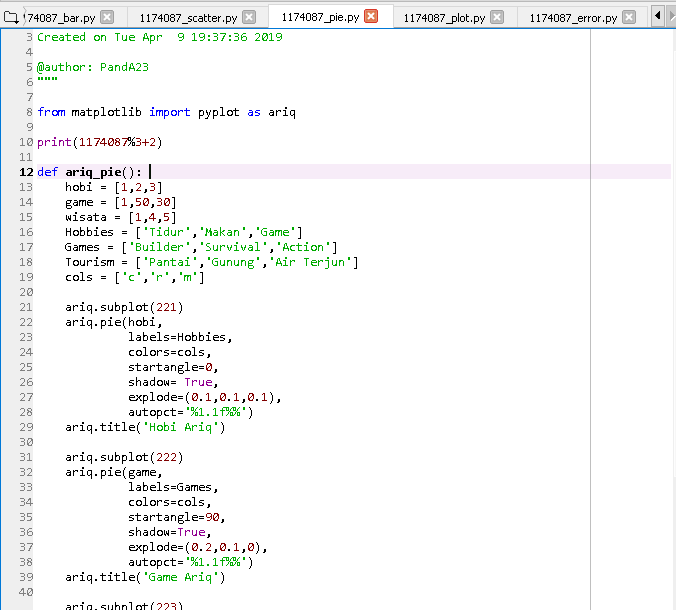
\includegraphics[width=7cm]{figures/6/1174087/Praktek/1174087_pie.png}
    \centering
    \caption{Pie}
\end{figure}

\begin{figure}[ht]	
    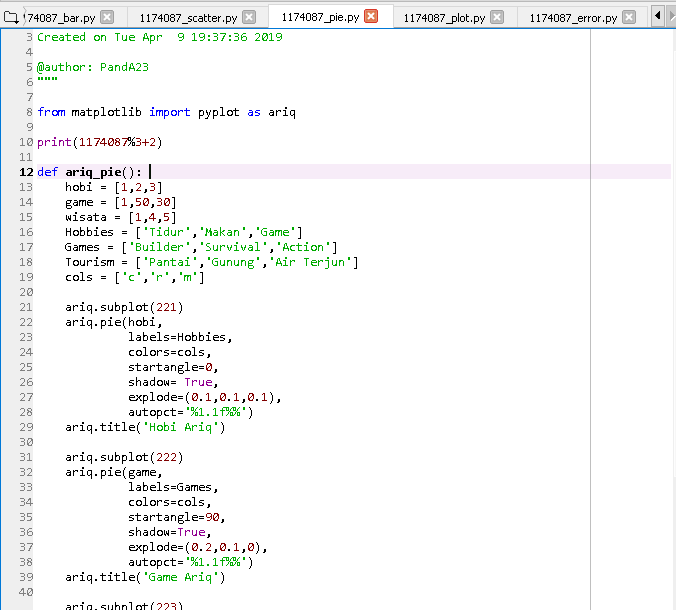
\includegraphics[width=7cm]{figures/6/1174087/Praktek/1174087_pie.png}
    \centering
    \caption{Plot}
\end{figure}

\begin{figure}[ht]	
    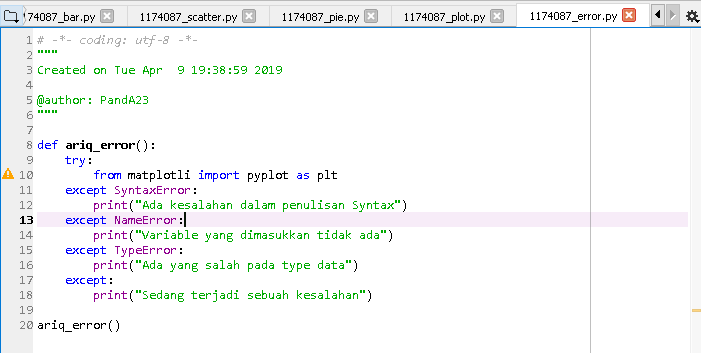
\includegraphics[width=7cm]{figures/6/1174087/Praktek/1174087_error.png}
    \centering
    \caption{Penanganan Error}
\end{figure}
%%%%%%%%%%%%%%%%%%%%%%%%%%%%%%%%%%%%%%%%%%%%%%%%%%%%%%%%%%%

\section{Muhammad Reza Syachrani / 1174084}
\subsection{Ketrampilan Pemrograman}
\subsubsection{Soal 1}
jawaban : \lstinputlisting[caption=Jawaban no.1, firstline=8, lastline=25, ]{src/6/1174084/Praktek/1174084_bar.py}

\subsubsection{Soal 2}
jawaban : \lstinputlisting[caption=Jawaban no.2, firstline=8, lastline=25, ]{src/6/1174084/Praktek/1174084_scatter.py}

\subsubsection{Soal 3}
jawaban : \lstinputlisting[caption=Jawaban no.3, firstline=8, lastline=49, ]{src/6/1174084/Praktek/1174084_pie.py}

\subsubsection{Soal 4}
jawaban : \lstinputlisting[caption=Jawaban no.4, firstline=8, lastline=25, ]{src/6/1174084/Praktek/1174084_plot.py}

\subsection{Ketrampilan Penanganan Error}
\begin{itemize}
\item ValueError adalah kesalahan dengan konten objek yang anda coba tetapkan nilainya. Solusinya adalah memperbaiki nilai dari objek.

\item NameError adalah exception saat kode melakukan eksekusi terhadap local name atau global name yang tidak terdefinisi atau tidak ada. Solusinya adalah memastikan variabel atau function yang akan dipanggil ada didalam program atau tidak salah mengetikannya.

\item Syntax Errors adalah kesalahan pada penulisan syntax atau kode. Solusinya adalah memperbaiki penulisan syntax atau kode


\lstinputlisting[caption=error, firstline=8, lastline=29, ]{src/6/1174084/Praktek/1174084_error.py}
\end{itemize}